\section{\'Eléments sur la simulation pseudo-aléatoire}\label{pseudoaleatoire}

Les générateurs pseudo-aléatoires sont des él\'ements central des m\'ethodes de simulation : elles reposent toutes sur la transformation de variables
uniformes $\mathcal{U}(0,1)$. \\

\begin{definition}{\bf G\'en\'erateur pseudo-al\'eatoire.}
Un \emph{g\'en\'erateur pseudo-al\'eatoire} est une transformation 
d\'eterministe $\Psi$ de $]0,1[$ dans $]0,1[$ telle que, pour toute valeur initiale $u_0$ et 
tout $n$, la suite 
$$
  \{ u_0,\Psi(u_0),\Psi(\Psi(u_0)),\ldots,\Psi^n(u_0) \}
$$
a le m\^eme comportement statistique qu'une suite iid $\mathcal{U}(0,1)$. 
\end{definition}

Sans appel au ``hasard", la suite d\'eterministe $(u_0,u_1=\Psi(u_0),
\ldots,u_n=\Psi(u_{n-1}))$\\ doit ressembler \`a une suite al\'eatoire.\\

\begin{itemize}
\item En {\bf Python}, il faut faire appel \`a la proc\'edure 
\texttt{ random.seed( )} \\

{\footnotesize 
{\sffamily

{\bfseries Description:}\\
'random.seed(a=None, version=2)' generates pseudo-random values with seed 'a'.

{\bfseries Exemple:}\\
    u = random.seed(20)

Generally, the seed value is the previous number generated by the generator. However, When the first time you use the random generator, there is no previous value. So by-default current system time is used as a seed value.} }\\

\begin{center}
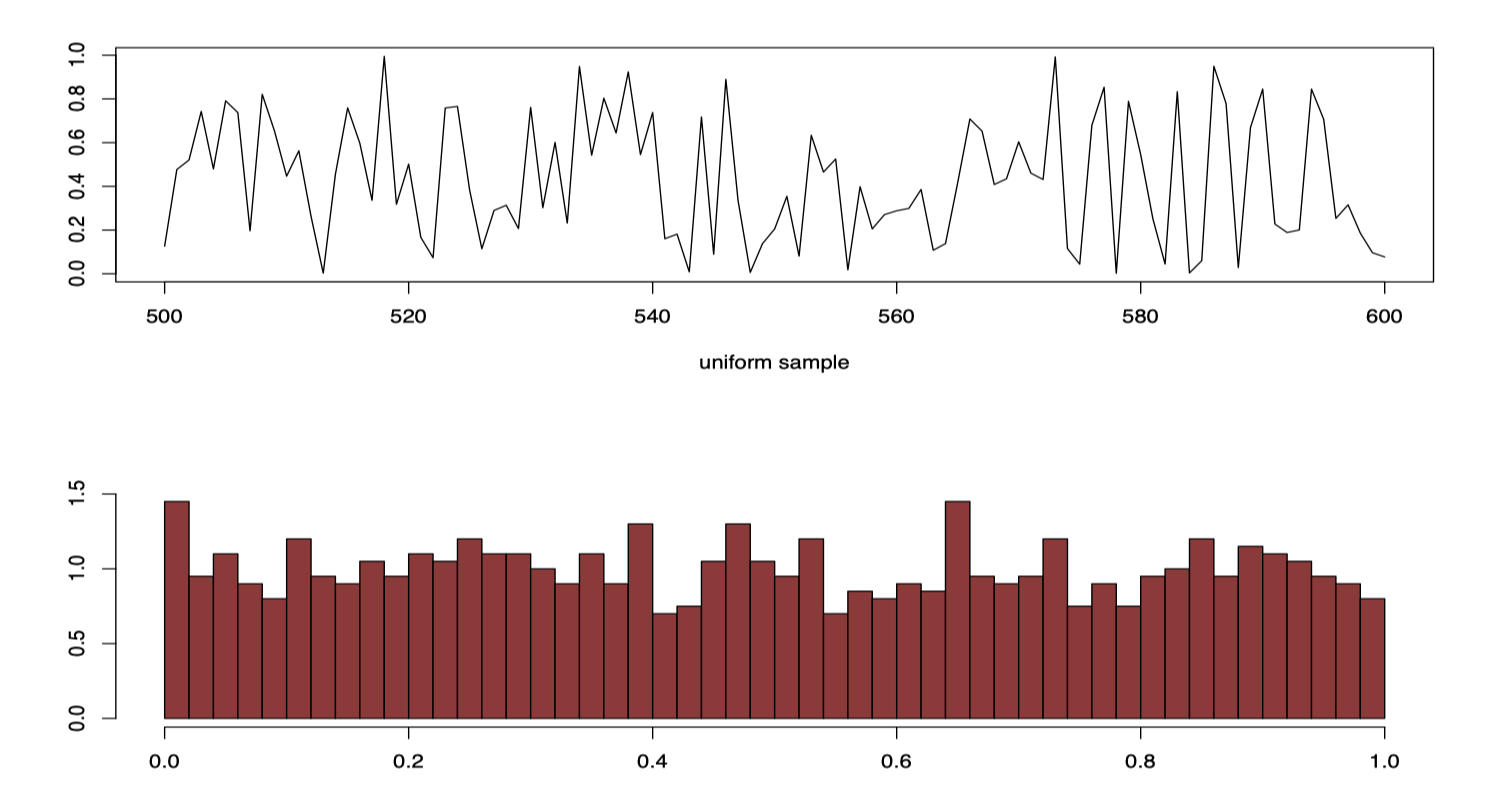
\includegraphics[scale=0.3]{figures/calcul/runif.png}
\end{center}


\item En {\bf C}, il faut faire appel \`a la proc\'edure \texttt{ rand()} / {\tt random()} \\

{\footnotesize 
{\sffamily

{\bfseries SYNOPSIS}\\
       \# include $<$stdlib.h$>$\\
       long int random(void);

{\bfseries DESCRIPTION}\\
The random() function uses a non-linear additive feedback 
random number generator employing a default table of size 
31 long integers to return successive pseudo-random numbers 
in the range from 0 to RAND MAX. The period of this random 
generator is very large, approximately 16*((2**31)-1).

{\bfseries RETURN VALUE}\\
random() returns a value between 0 and RAND MAX.}} \\
\end{itemize}

Un générateur usuel est le suivant :

\begin{definition}{Générateur congruenciel}
Le g\'en\'erateur congruenciel
$$
   D(x) = (ax + b) \; {\mathrm {mod}} \; (M+1) .
$$
est de p\'eriode $M$ pour les bons choix de $(a,b)$ et se transforme en
g\'en\'erateur sur $]0,1[$ par division par $M+2$. \\
\end{definition}


\begin{center}
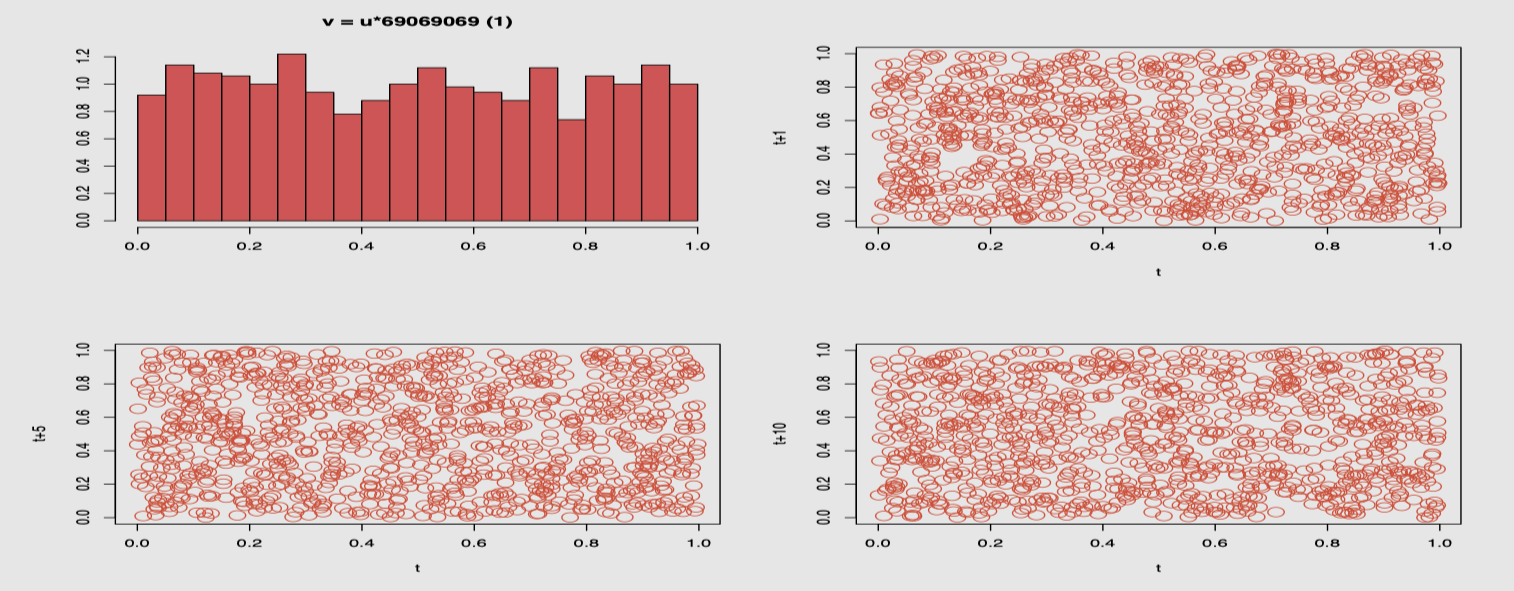
\includegraphics[scale=0.3]{figures/calcul/congru.png}
\end{center}

Il faut toujours utiliser la fonction appropri\'ee sur l'ordinateur ou le logiciel en service
plut\^ot que de construire un g\'en\'erateur al\'eatoire de mauvaise qualit\'e. 